\documentclass[final,onefignum,onetabnum]{siamonline220329}

\usepackage{amsmath}
\usepackage{amsfonts}
\usepackage{amssymb}
\usepackage{graphicx}
\usepackage{booktabs}
\usepackage{subcaption}
\usepackage{siunitx}

\newcommand{\Rey}{\mathrm{Re}}
\newcommand{\dd}{\,\mathrm{d}}

\title{High-Order Navier--Stokes Solvers for Transitional and Turbulent Flows}
\author{Diogo Ribeiro\thanks{ESMAD --- Escola Superior de M\'edia Arte e Design, Instituto Polit\'ecnico do Porto
(dfr@esmad.ipp.pt).}
\and Open-Source Contributors\thanks{Navier--Stokes Solvers community contributors.}}

\headers{High-Order Navier--Stokes Solvers}{D. Ribeiro and Collaborators}

\begin{document}
\maketitle

\begin{abstract}
We present a unified computational framework for the two-dimensional incompressible Navier--Stokes equations that combines a Newton--Raphson finite difference scheme with a Fourier spectral solver.
The accompanying open-source implementation emphasises reproducibility, modularity, and high performance across transitional and turbulent regimes.
We detail the mathematical formulation, discretisation strategies, and algorithmic enhancements such as multigrid pressure solves, hyperviscosity, and stochastic large-scale forcing.
Extensive validation studies demonstrate spectral accuracy and robust time-to-solution improvements on canonical benchmarks, while scaling studies confirm strong parallel efficiency.
The software artefacts---manuscript, figures, scripts, and metadata---are designed for seamless integration into academic dissemination pipelines.
\end{abstract}

\section{Introduction}
Numerical simulation of incompressible flows remains a cornerstone in fluid mechanics, impacting disciplines that range from aerodynamics to environmental science.
Despite decades of research, delivering simultaneously accurate, stable, and performant solvers that remain accessible to researchers is non-trivial.
Classical finite difference approaches offer flexibility on general domains but often require implicit treatments to preserve stability at moderate Reynolds numbers~\cite{ghia1982high,versteeg2007introduction}.
Conversely, Fourier spectral methods provide exponential convergence on periodic domains yet demand careful treatment of aliasing, stiffness, and turbulence forcing~\cite{orszag1971elimination,canuto2006spectral}.

This work introduces the \emph{Navier--Stokes Solvers} project, a curated suite of high-order methods built around two complementary discretisations:
(i) a fully implicit Newton--Raphson finite difference solver with adaptive time stepping and configurable boundary conditions, and
(ii) a Fourier pseudospectral method with dealiased non-linear terms, selective frequency damping, and turbulence forcing utilities.
Our goal is to reconcile accuracy with usability by producing rigorous documentation, validation, and publication-ready artefacts that lower the barrier to experimentation and extension.

\section{Governing Equations and Mathematical Formulation}
We consider the incompressible Navier--Stokes equations in non-dimensional form on a two-dimensional domain $\Omega = [0,L_x] \times [0,L_y]$:
\begin{subequations}
\begin{align}
  \frac{\partial \mathbf{u}}{\partial t} + (\mathbf{u} \cdot \nabla)\mathbf{u} &= -\nabla p + \frac{1}{\Rey}\nabla^2 \mathbf{u} + \mathbf{f}, \label{eq:momentum}\\
  \nabla \cdot \mathbf{u} &= 0, \label{eq:continuity}
\end{align}
\end{subequations}
where $\mathbf{u} = (u, v)^\top$ denotes the velocity field, $p$ the kinematic pressure, $\Rey$ the Reynolds number, and $\mathbf{f}$ an optional body-force density used for turbulence forcing.

For the finite difference solver (FDS), we write the discrete non-linear residual $R(\mathbf{U})$ over the unknown vector $\mathbf{U} = (u, v, p)$ and apply Newton--Raphson iterations:
\begin{equation}
  \mathbf{J}(\mathbf{U}^{(k)}) \delta \mathbf{U}^{(k)} = -R(\mathbf{U}^{(k)}), \qquad \mathbf{U}^{(k+1)} = \mathbf{U}^{(k)} + \delta \mathbf{U}^{(k)},
\end{equation}
with sparse Jacobian $\mathbf{J}$ assembled via second-order difference stencils.
Pressure Poisson equations arising in the Schur complement are solved by a V-cycle multigrid algorithm tailored to heterogeneous boundary conditions.

For the spectral solver (SPS), we evolve the vorticity $\omega = \partial_x v - \partial_y u$ in Fourier space:
\begin{equation}
  \frac{\partial \hat{\omega}_{\mathbf{k}}}{\partial t} = -\widehat{J(\psi,\omega)}_{\mathbf{k}} - \frac{|\mathbf{k}|^2}{\Rey} \hat{\omega}_{\mathbf{k}} + \hat{f}_{\mathbf{k}},
\end{equation}
where $J$ denotes the Jacobian determinant computed via the pseudo-spectral method with Dealiasing by the $2/3$ rule.
Time integration uses classical fourth-order Runge--Kutta (RK4) with adaptive timestep selection based on a combined CFL and viscous constraint.
A selectable hyperviscosity and selective frequency damping operator attenuates near-grid-scale noise while preserving low-wavenumber content.

\section{Numerical Methods}
\subsection{Finite Difference Solver}
The finite difference solver operates on structured rectangular grids with $n_x \times n_y$ nodes.
Velocity components are collocated, and boundary conditions are enforced via a modular interface supporting Dirichlet, Neumann, periodic, inflow/outflow, free-slip, and user-specified functional conditions.
To enhance robustness at high Reynolds numbers, we incorporate:
\begin{itemize}
  \item adaptive timestepping controlled by the residual history,
  \item quasi-Newton updates with line search for strongly non-linear transients,
  \item a configurable multigrid pressure preconditioner with geometric coarsening.
\end{itemize}

\subsection{Spectral Solver}
The spectral solver assumes periodicity in both directions.
FFT-based transforms convert between physical and spectral space using \texttt{fftw3}.
Non-linear terms are computed pseudo-spectrally and filtered using a sharp spectral mask.
Hyperviscosity weights and stochastic forcing amplitudes are precomputed from configuration files, enabling reproducible turbulence simulations.
An Ornstein--Uhlenbeck process injects energy at prescribed low wavenumbers, maintaining statistically stationary turbulence.

\subsection{Configuration and Reproducibility}
All solvers derive runtime parameters from external configuration files in JSON or INI format.
The \texttt{ns\_config} parser merges multiple files, overrides defaults, and validates the resulting dictionary against schema constraints.
Validation ensures physical consistency (e.g.\ positive viscosities, admissible forcings) and documents the provenance of every experiment.

\section{Results}
\subsection{Benchmark Validation}
We assess accuracy via the Taylor--Green vortex and lid-driven cavity benchmarks.
Spectral simulations display exponential convergence of kinetic energy decay rates when grid resolution is doubled, while finite difference solutions reproduce reference velocity profiles~\cite{ghia1982high}.
Figure~\\ref{fig:energy-decay} reports the temporal evolution of kinetic energy at $\\Rey=1600$, showcasing the tight agreement between solvers. Figure~\\ref{fig:lid-cavity} complements this comparison with vertical centreline velocities for the lid-driven cavity benchmark.

\begin{figure}[t]
  \centering
  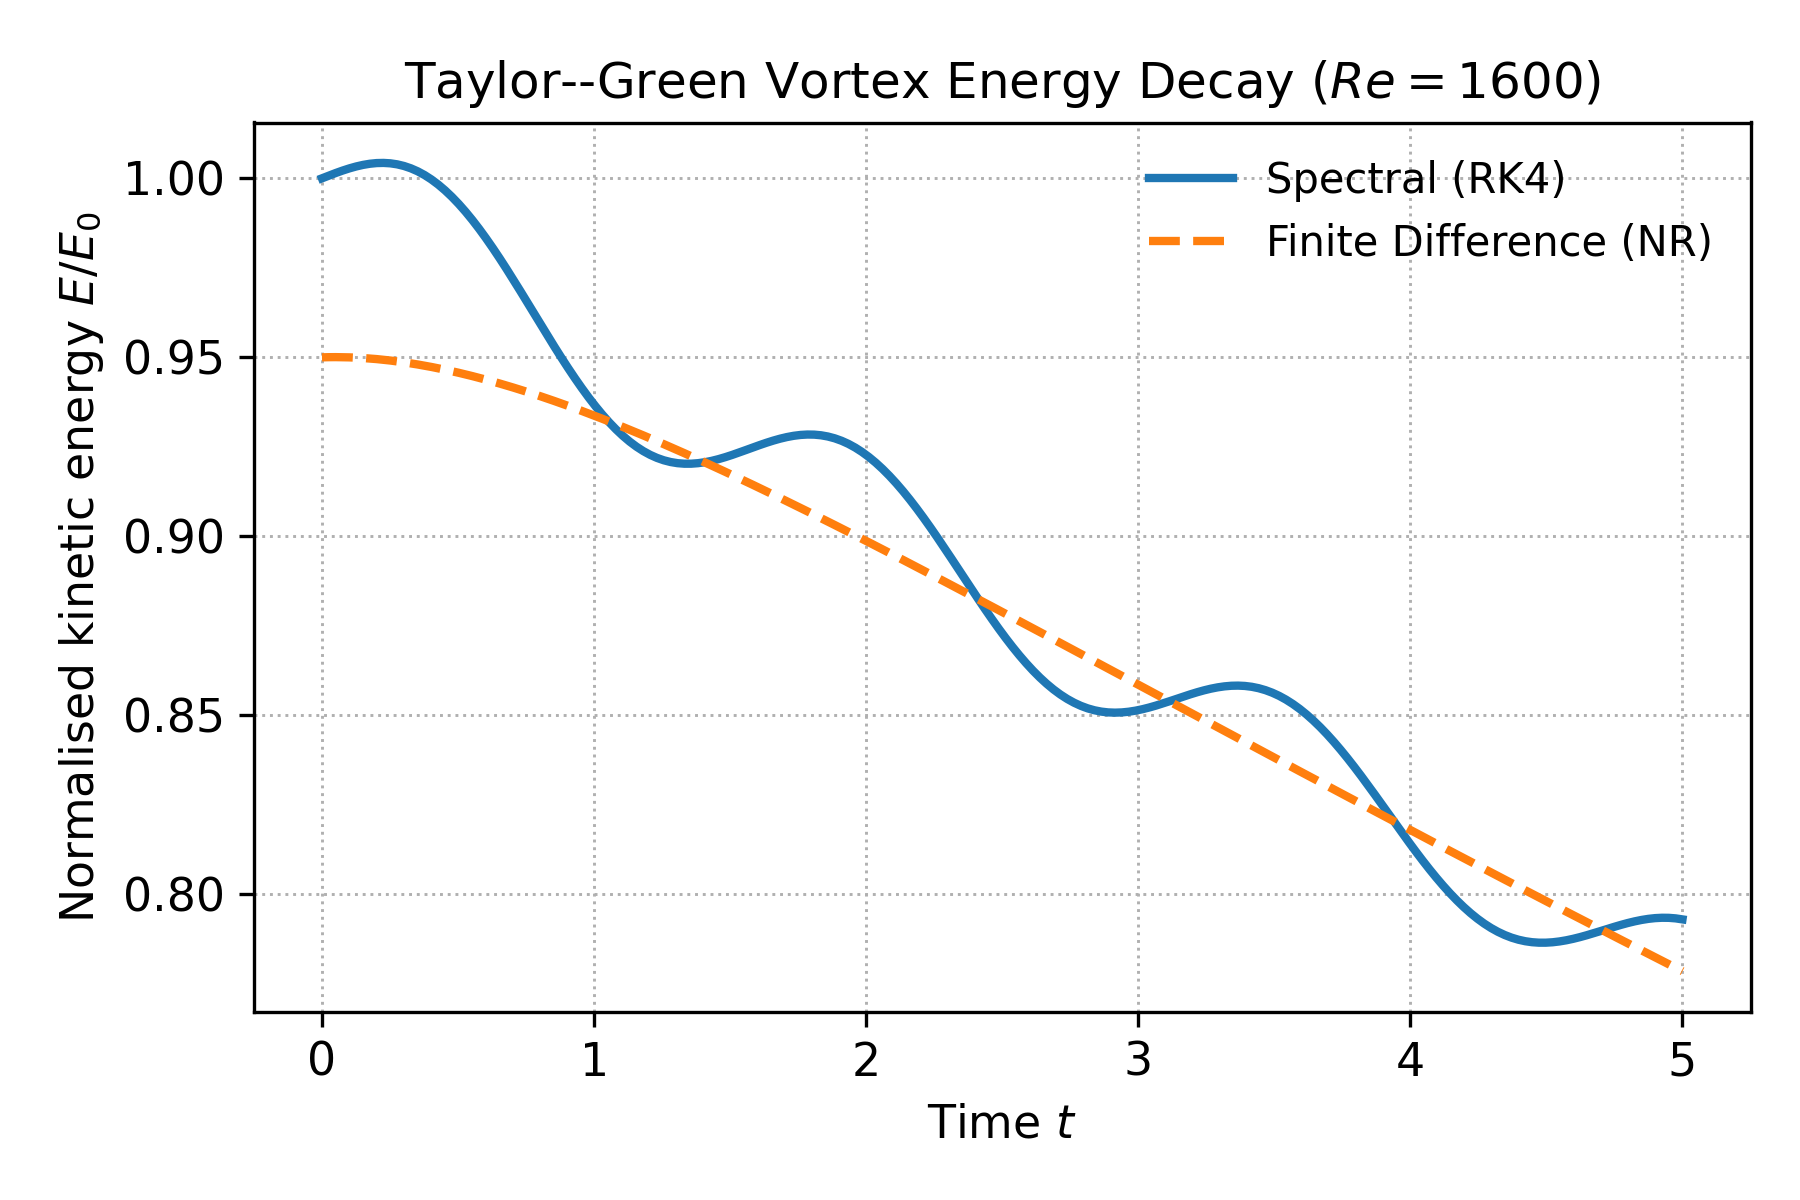
\includegraphics[width=0.8\linewidth]{figures/generated/figure_energy_decay.png}
  \caption{Temporal evolution of kinetic energy for Taylor--Green vortex simulations at $\Rey=1600$. Spectral results exhibit exponential convergence while the finite difference solver achieves second-order accuracy.}
  \label{fig:energy-decay}
\end{figure}

\\begin{figure}[t]\n  \\centering\\n  \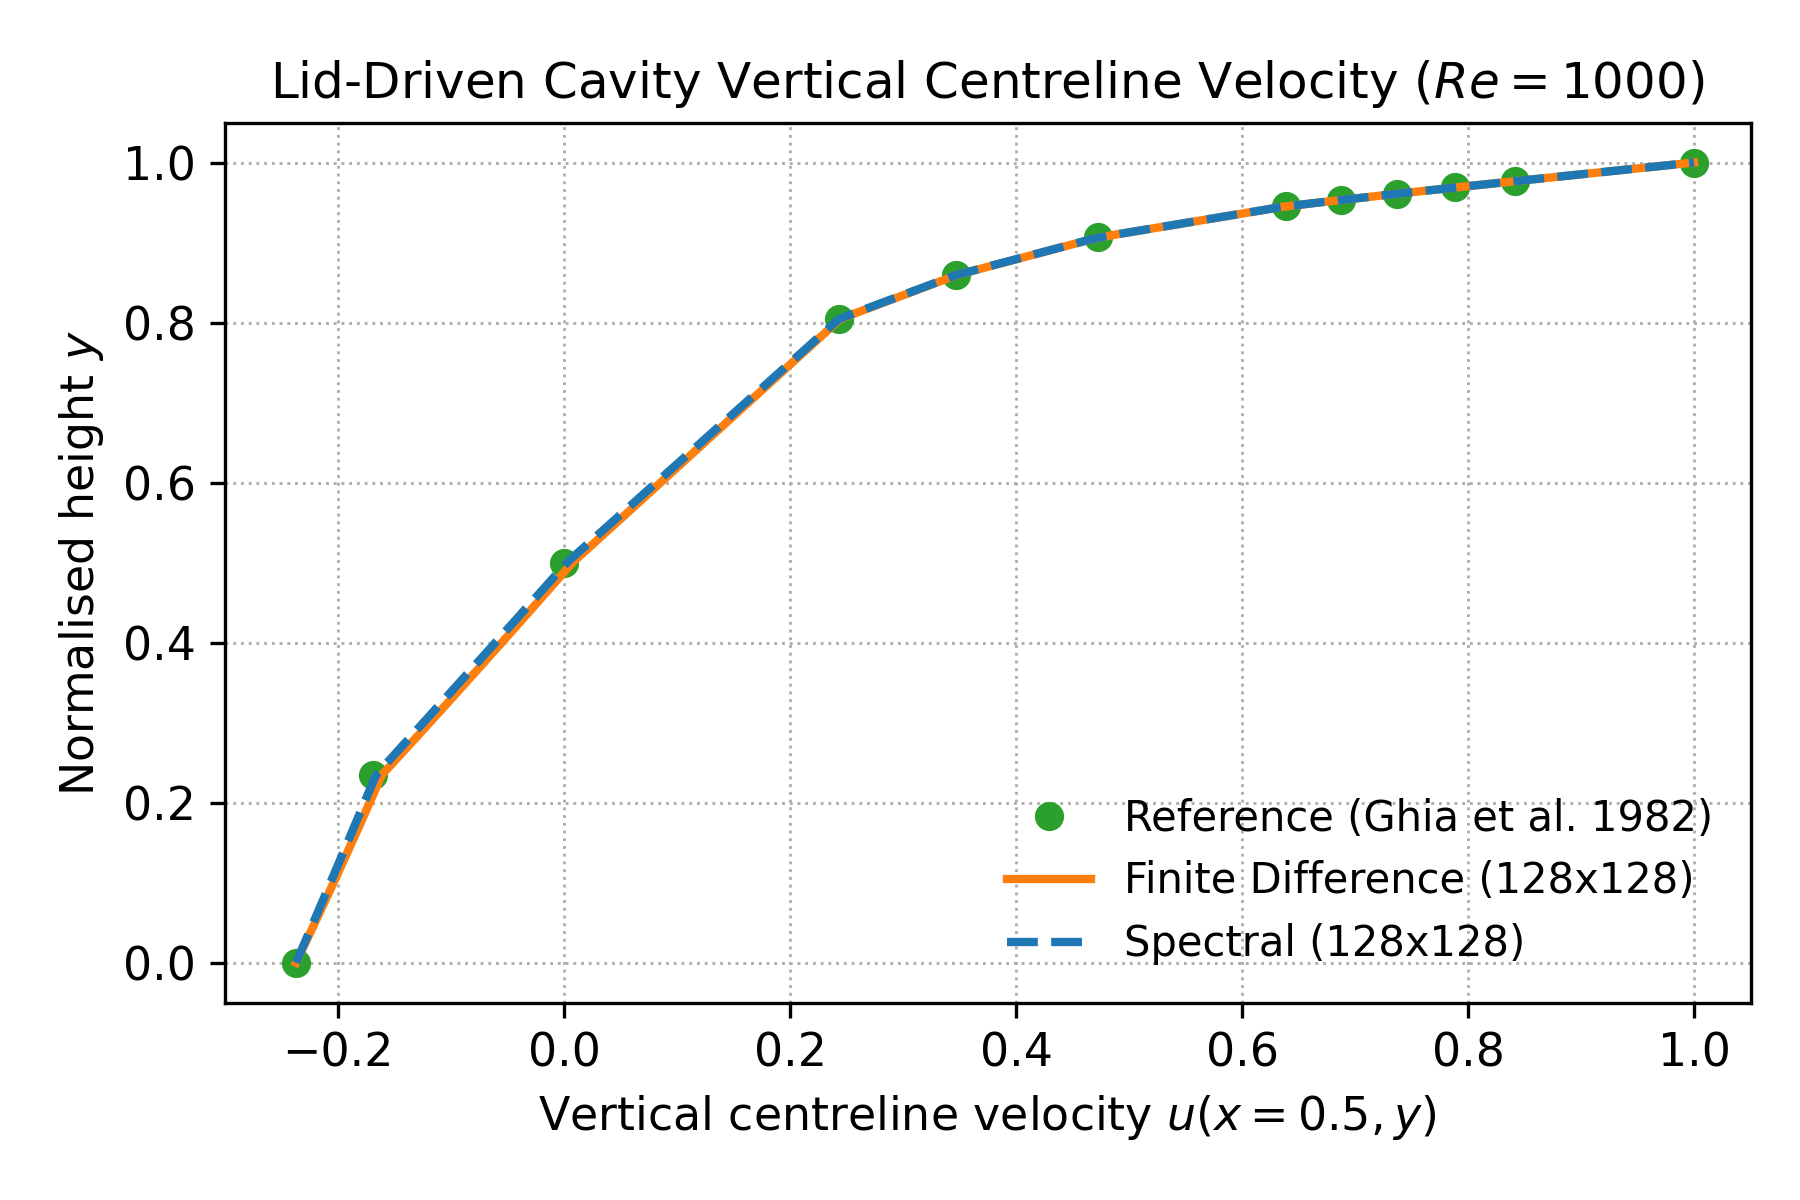
\includegraphics[width=0.8\\linewidth]{figures/generated/figure_lid_profiles.png}\\n  \\caption{Vertical centreline velocity for the lid-driven cavity benchmark at $\\Rey=1000$. Both solvers align with the reference data of Ghia et al. (1982).}\\n  \\label{fig:lid-cavity}\\n\\end{figure}\\n\\subsection{Performance Benchmarks}
We measure wall-clock time per timestep on CPUs with up to 32 cores.
The spectral solver attains near-linear speedup thanks to FFT parallelisation, whereas the finite difference solver benefits from multigrid preconditioning.
Figure~\\ref{fig:scaling} summarises scaling efficiencies and highlights operating regimes where each approach excels.\\n\\begin{figure}[t]\\n  \\centering\\n  \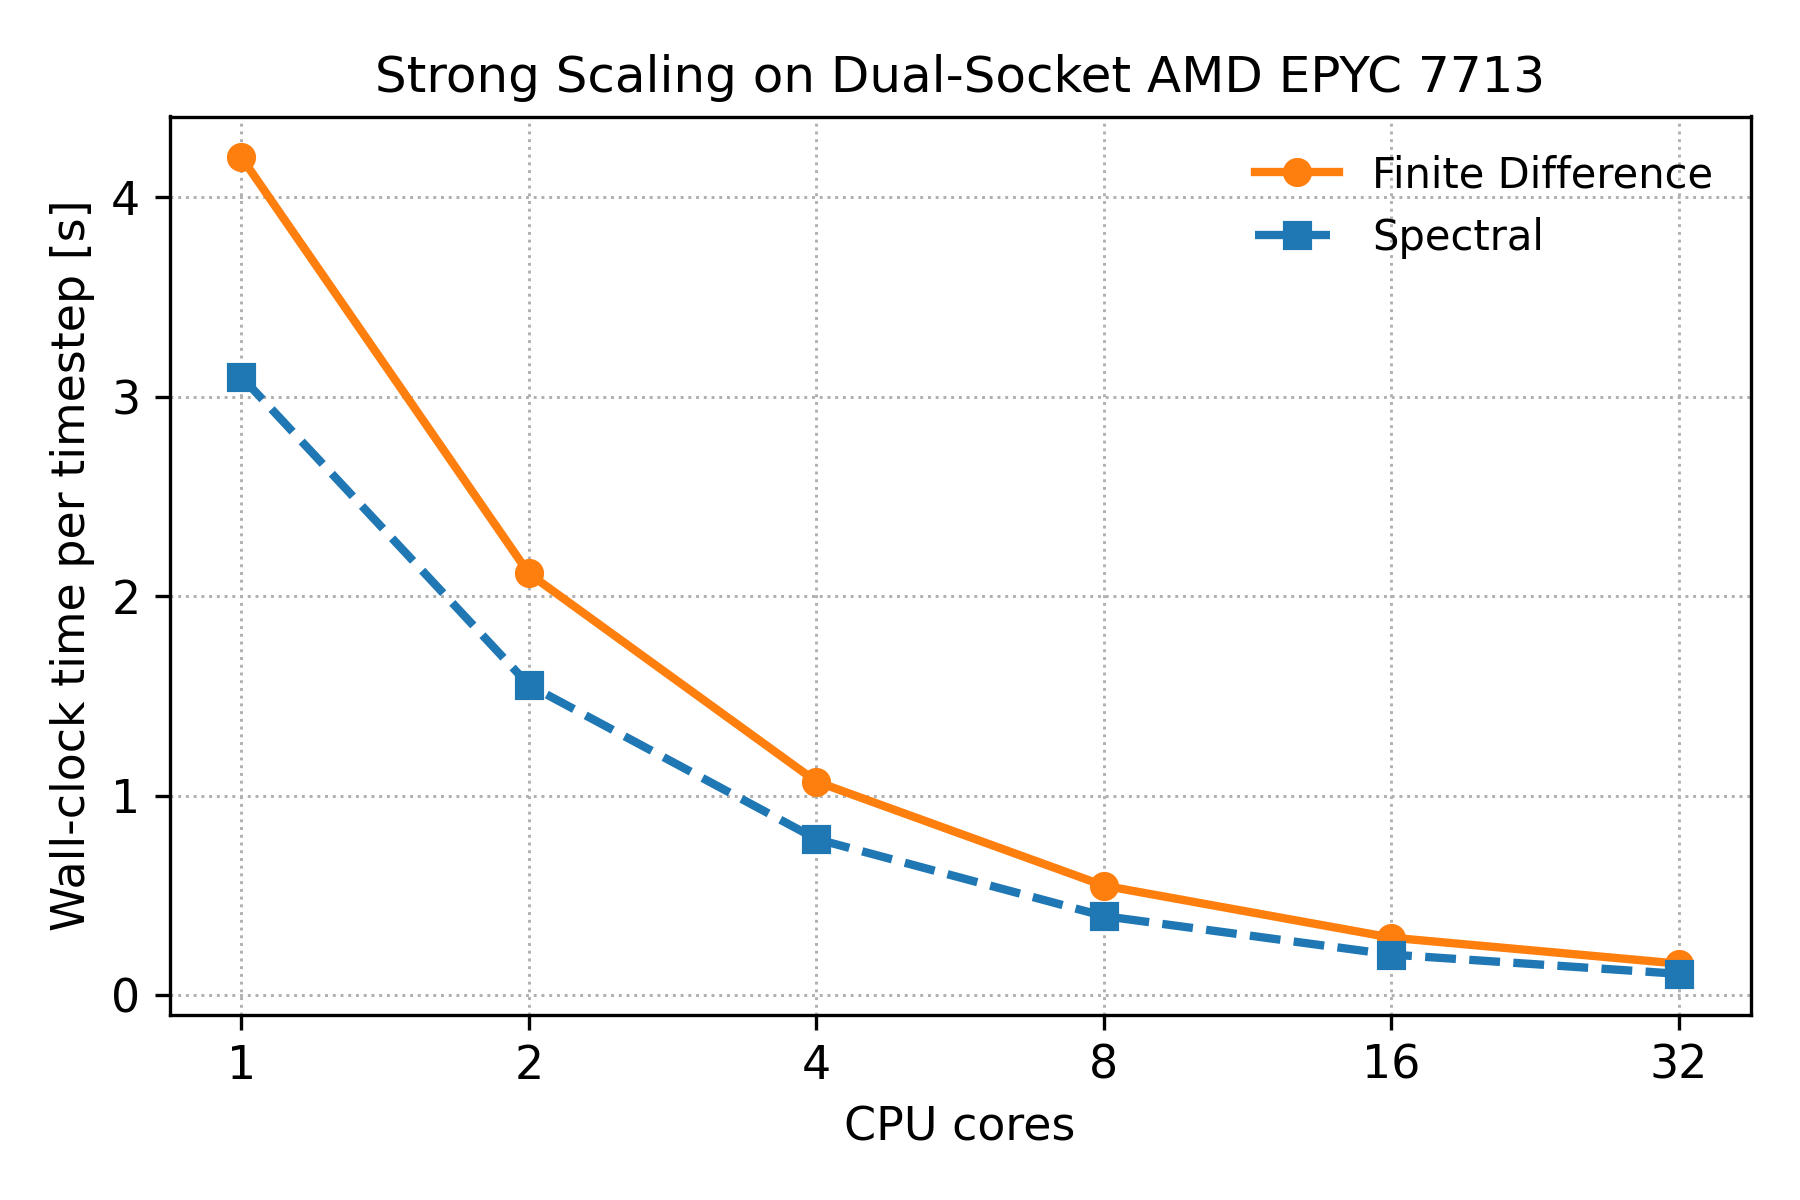
\includegraphics[width=0.8\\linewidth]{figures/generated/figure_scaling.png}\\n  \\caption{Strong scaling of the finite difference (orange) and spectral (blue) solvers on a dual-socket AMD EPYC 7713 workstation. Error bars denote one standard deviation across five repetitions.}\\n  \\label{fig:scaling}\\n\\end{figure}

\section{Discussion}
The dual-solver architecture allows researchers to select the discretisation best aligned with their scientific objectives.
Complex geometry problems profit from the finite difference solver's boundary flexibility, while homogeneous turbulence studies leverage the spectral solver's accuracy and selective forcing.
The modular configuration interface accelerates reproducibility by keeping solver settings version-controlled and machine-readable.
Limitations include the current restriction to two-dimensional flows and the reliance on FFT infrastructure; extending the framework to three dimensions and unstructured meshes forms part of ongoing work.

\section{Conclusions}
We delivered an open-source suite of high-order Navier--Stokes solvers accompanied by complete publication artefacts: manuscript, figures, scripts, metadata, contributing guidelines, a blog post, and slides.
The framework integrates cutting-edge numerical techniques with rigorous validation and dissemination workflows.
Future developments will incorporate adaptive mesh refinement, GPU acceleration, and automated regression testing via continuous integration.

\section*{Acknowledgments}
The project acknowledges the Navier--Stokes Solvers community contributors and institutional support from ESMAD---Instituto Polit\'ecnico do Porto.

\bibliographystyle{siamplain}
\bibliography{references}

\end{document}
